\chapter{Hauptteil}

\blindtext

\section{Zitate}

Zitieren ist leicht in \LaTeX{}. Zitiert werden können Bücher \cite{fitzgerald:realigning_research_and_practice}, Internetquellen \cite{stallman99:telepolis}, Konferenzbände \cite{raymond:cathedral_bazaar_book} und noch vieles mehr. Zitierte Quellen werden automatisch ins Literaturverzeichnis übernommen.

\section{Abbildungen}

\begin{figure}[H]
	\centering
	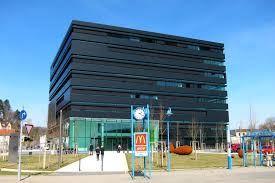
\includegraphics[keepaspectratio]{./bilder/dhbw.jpg}
	\caption{DHBW Heidenheim}
	\label{dhbwhdh}
\end{figure}

Diese Abbildung kommt automatisch ins Abbildungsverzeichnis. Man kann Abbildungen wie die Abbildung \ref{dhbwhdh} auch referenzieren.

\section{Tabellen}

\begin{table}[H]
	\begin{center}
		\begin{tabular}{l|c|r}
			\toprule
			\textbf{Wert 1} & \textbf{Wert 2} & \textbf{Wert 3}\\
			$\alpha$ & $\beta$ & $\gamma$ \\
			\midrule
			1 & 1110.1 & a\\
			2 & 10.1 & b\\
			3 & 23.113231 & c\\
			\bottomrule
		\end{tabular}
	\caption{Meine Tabelle}
	\label{tabelle}
	\end{center}
\end{table}

Eine Tabelle erscheint automatisch im Tabellenverzeichnis. Auch eine Tabelle wie die Tabelle \ref{tabelle} kann problemlos referenziert werden.

\section{Mathe im Text}

\blindmathtrue
\blindtext

\section{Mathe}

\blindmathfalse
\blindmathpaper

\subsection{Formeln mit Nummerierung}

\blindtext

\begin{equation}
	a=x^2+5*y
	\label{randomformel}
\end{equation}

Es ist auch möglich Formeln zu referenzieren. Formel \ref{randomformel} ist nur eine zufällige Formel.

\subsection{Formeln ohne Nummerierung}

\blindtext

\begin{equation*}
	b=z^2+3*p
\end{equation*}

\subsubsection{Das ist eine Subsubsection}

\blindtext